\documentclass[12pt, letterpaper]{article}
\usepackage[utf8]{inputenc}
\usepackage[left = 2.5cm, right = 2.5cm, top = 2.5cm, bottom = 2.5cm]{geometry}
\usepackage{amsthm}
\usepackage{amsfonts}
\usepackage{amsmath}
\usepackage{amssymb}
\usepackage{graphicx}
\usepackage[T1]{fontenc}
\usepackage{listings}
\graphicspath{{images/}}



\author{Hernández Ferreiro Enrique Ehecatl \\
        López Soto Ramses Antonio \\
        Miguel Torres Eric Giovanni \\
        Quintero Villeda Erik}

\title{Práctica 5 \\
       {\small Fudamentos de Bases de Datos}}

\date{23 de septiembre de 2019}

\begin{document}
    \maketitle

    \section*{Introducción}

        \subsection*{Objetivo}
        Crear una esquema de base de datos haciendo uso de restricciones.

    \section*{Desarrollo}
    A partir del \textit{Modelo Relacional} que adaptamos en prácticas anteriores: \vspace{.2cm}

    \begin{center}
        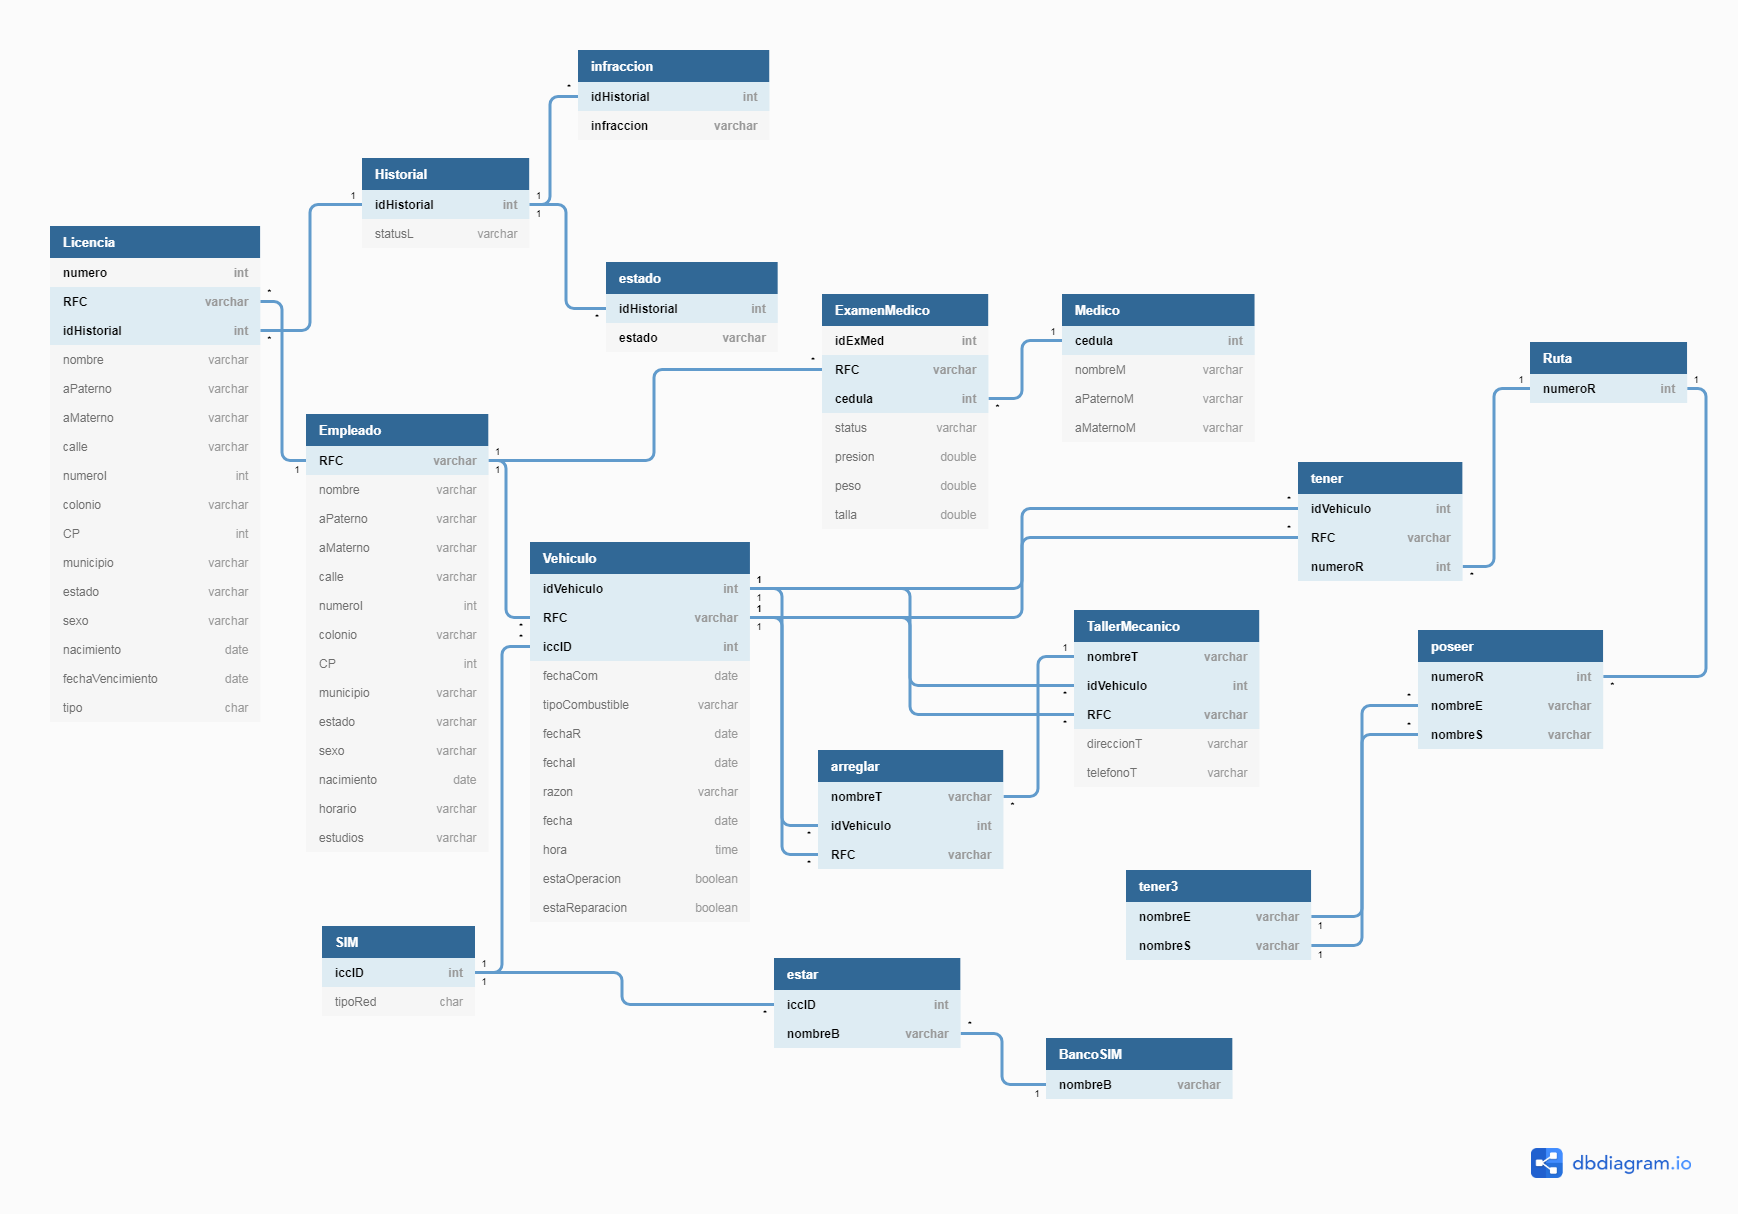
\includegraphics[scale=0.2]{CasPrueba.png}
    \end{center}

    Basándonos en el esquema anterior, el esquema en \textit{SQL} se ve como sigue: \vspace{.3cm}
    
    { \tiny
    \begin{lstlisting}
        CREATE DATABASE MovilidadCDMX;
        GO

        CREATE TABLE MovilidadCDMX.dbo.Empleado (
            RFC varchar(13) PRIMARY KEY,
            nombre varchar(20) NULL,
            aPaterno varchar(20) NULL,
            aMaterno varchar(20) NULL,
            calle varchar(20) NOT NULL,
            numeroI int NOT NULL,
            cp int NOT NULL,
            colonia varchar(20) NULL,
            municipio varchar(20) NOT NULL,
            estado varchar(20) NOT NULL,
            sexo varchar(10) NOT NULL,
            nacimiento datetime NULL,
            horario time NOT NULL,
            estudios varchar(15) NULL
        ) 	
        GO


        CREATE TABLE MovilidadCDMX.dbo.Historial (
            idHistorial int PRIMARY KEY,
            statusL varchar(10) NULL
        ) 
        GO


        CREATE TABLE MovilidadCDMX.dbo.Licencia (
            numero int PRIMARY KEY,
            RFC varchar(13),
            idHistorial int,
            nombre varchar(20) NULL,
            aPaterno varchar(20) NULL,
            aMaterno varchar(20) NULL,
            calle varchar(20) NOT NULL,
            numeroI int NOT NULL,
            cp int NOT NULL,
            colonia varchar(20) NOT NULL,
            municipio varchar(20) NOT NULL,
            estado varchar(20) NOT NULL,
            sexo varchar(10) NOT NULL,
            nacimiento datetime NULL,
            fechaVencimiento datetime NOT NULL,
            tipo char(1) NOT NULL,
            CONSTRAINT FK_Empleado FOREIGN KEY (RFC) REFERENCES MovilidadCDMX.dbo.Empleado (RFC),
            CONSTRAINT FK_Historia FOREIGN KEY (idHistorial) REFERENCES MovilidadCDMX.dbo.Historial (idHistorial)
        ) 
        GO

        CREATE TABLE MovilidadCDMX.dbo.infraccion (
            idHistorial int,
            infraccion varchar(20) PRIMARY KEY,
            CONSTRAINT FK_Historial2 FOREIGN KEY (idHistorial) REFERENCES MovilidadCDMX.dbo.Historial (idHistorial)
        ) 
        GO


        CREATE TABLE MovilidadCDMX.dbo.estado (
            idHistorial int,
            estado varchar(20) PRIMARY KEY,
            CONSTRAINT FK_Historial3 FOREIGN KEY (idHistorial) REFERENCES MovilidadCDMX.dbo.Historial (idHistorial)
        ) 
        GO


        CREATE TABLE MovilidadCDMX.dbo.SIM (
            iccID int PRIMARY KEY,
            tipoRed char(1) NOT NULL
        ) 
        GO


        CREATE TABLE MovilidadCDMX.dbo.Vehiculo (
            idVehiculo int PRIMARY KEY,
            RFC varchar(13),
            iccID int,
            fechaCom datetime NOT NULL,
            tipoCombustible varchar(10) NOT NULL,
            fechaR datetime NOT NULL,
            fechaI datetime NOT NULL,
            razon varchar(30) NULL,
            fecha datetime NOT NULL,
            hora time NULL,
            estaOperacion char(2) NOT NULL,
            estaReparacion char(2) NOT NULL,
            CONSTRAINT FK_Empleado2 FOREIGN KEY (RFC) REFERENCES MovilidadCDMX.dbo.Empleado (RFC),
            CONSTRAINT FK_SIM FOREIGN KEY (iccID) REFERENCES MovilidadCDMX.dbo.SIM (iccID)
        ) 
        GO


        CREATE TABLE MovilidadCDMX.dbo.BancoSIM (
            nombreB varchar(20) PRIMARY KEY
        ) 
        GO


        CREATE TABLE MovilidadCDMX.dbo.estar (
            iccID int,
            nombreB varchar(20) NOT NULL,
            CONSTRAINT FK_SIM2 FOREIGN KEY (iccID) REFERENCES MovilidadCDMX.dbo.SIM (iccID),
            CONSTRAINT FK_BancoSIM FOREIGN KEY (nombreB) REFERENCES MovilidadCDMX.dbo.BancoSIM (nombreB)
        ) 
        GO


        CREATE TABLE MovilidadCDMX.dbo.Medico (
            cedula int PRIMARY KEY,
            nombreM varchar(20) NULL,
            aPaternoM varchar(15) NULL,
            aMaternoM varchar(15) NULL
        ) 
        GO


        CREATE TABLE MovilidadCDMX.dbo.ExamenMedico (
            idExMed int PRIMARY KEY,
            RFC varchar(13),
            cedula int,
            status varchar(10) NULL,
            presion float NULL,
            peso float NULL,
            talla float NULL,
            CONSTRAINT FK_Empleado3 FOREIGN KEY (RFC) REFERENCES MovilidadCDMX.dbo.Empleado (RFC),
            CONSTRAINT FK_Medico FOREIGN KEY (cedula) REFERENCES MovilidadCDMX.dbo.Medico (cedula)
        ) 
        GO


        CREATE TABLE MovilidadCDMX.dbo.TallerMecanico (
            nombreT varchar(20) PRIMARY KEY,
            idVehiculo int,
            RFC varchar(13),
            direccionT varchar(50) NOT NULL,
            telefonoT int NOT NULL
            CONSTRAINT FK_Vehiculo2 FOREIGN KEY (idVehiculo) REFERENCES MovilidadCDMX.dbo.Vehiculo (idVehiculo),
            CONSTRAINT FK_Emp2 FOREIGN KEY (RFC) REFERENCES MovilidadCDMX.dbo.Empleado (RFC)
        ) 
        GO


        CREATE TABLE MovilidadCDMX.dbo.arreglar (
            nombreT varchar(20),
            idVehiculo int ,
            RFC varchar(13),
            CONSTRAINT FK_Vehiculo FOREIGN KEY (idVehiculo) REFERENCES MovilidadCDMX.dbo.Vehiculo (idVehiculo),
            CONSTRAINT FK_TallerMecanico FOREIGN KEY (nombreT) REFERENCES MovilidadCDMX.dbo.TallerMecanico (nombreT),
            CONSTRAINT FK_Emp FOREIGN KEY (RFC) REFERENCES MovilidadCDMX.dbo.Empleado (RFC)
        ) 
        GO


        CREATE TABLE MovilidadCDMX.dbo.Ruta (
            numeroR int PRIMARY KEY
        ) 
        GO


        CREATE TABLE MovilidadCDMX.dbo.tener (
            idVehiculo int,
            RFC varchar(13),
            numeroR int,
            CONSTRAINT FK_Vehiculo4 FOREIGN KEY (idVehiculo) REFERENCES MovilidadCDMX.dbo.Vehiculo (idVehiculo),
            CONSTRAINT FK_Emp3 FOREIGN KEY (RFC) REFERENCES MovilidadCDMX.dbo.Empleado (RFC),
            CONSTRAINT FK_Ruta FOREIGN KEY (numeroR) REFERENCES MovilidadCDMX.dbo.Ruta (numeroR)
        ) 
        GO


        CREATE TABLE MovilidadCDMX.dbo.tener3 (
            nombreE varchar(15) PRIMARY KEY
        ) 
        GO

        CREATE TABLE MovilidadCDMX.dbo.poseer (
            numeroR int,
            nombreE varchar(15),
            nombreS varchar(15) NOT NULL,
            CONSTRAINT FK_Rutas FOREIGN KEY (numeroR) REFERENCES MovilidadCDMX.dbo.Ruta (numeroR),
            CONSTRAINT FK_tener3 FOREIGN KEY (nombreE) REFERENCES MovilidadCDMX.dbo.tener3 (nombreE),
        ) 
        GO
    \end{lstlisting}}

    Para la implementación del esquema anterior, hicimos uso de los tipos de datos y restrcciones requeridas para cada uno de los atributos de las tablas.

    \section*{Conclusiones}
    Nos tardamos alrededor de 4 horas en terminar de implementar el esquema de la base de datos, pues ninguno de los cuatro
    estaba muy familiarizado con el lenguaje $T-SQL$, por lo que nos costó un poco de trabajo, al principio, entenderlo. \vspace{.3cm}

    En resumen, el lenguaje $T-SQL$ puede llegar a ser un poco delicado pues, al ser ejecutado de manera secuencial, se debe tener
    mucho cuidado en la forma en la cual se definen las tablas con sus respectivas restricciones.
    
\end{document}
